ArcGIS along with other GIS programs are capable of importing \netcdf~files - a
common format for saving multi-dimensional data.  In this tutorial however, we
are dealing with \ioapi~files.  \ioapi~is a wrapper format for \netcdf~files
produced by the \ac{bams} organization and is used by \ac{cmaq}, the
\ac{usepa}'s \acf{ctm}.

This wrapper imposes stricter condition on how data is saved in the files and
defines a custom header.  Unfortunately however, the \ioapi~headers are not compatible
with \netcdf's CF Conventions - the convention on how data in
\netcdf~files is, among other things, spatially referenced.  As a
result, \ioapi~files can still be imported using the Multidimensional
Toolbox in ArcGIS, however that data can not easily be spatially
referenced.

To compensate for this, I have developed a ArcGIS toolbox
(\textbf{AQM} $\rightarrow$ \textbf{Make IOAPI Raster File}) that
repairs the spatial information in the \ioapi~file.  This section
describes in detail how this tool functions.

Accessing \ioapi~files typically requires installing a long list of open source
software that has to be built from source on the host computer.  For the
purposes of a tool that can be shared, this was deemed extremely
impractical\footnote{Building this software typically takes members in our
research group months on Linux/Unix systems - the OS's that these systems are
best supported.  Installing these on Windows with Visual C++ is not feasible to
require in a shared ArcGIS toolbox.}.  Therefore the \ioapi~operations are
performed remotely via a webservice.

How this works? Once the \ioapi~file is uploaded and then
re-downloaded with the spatial information properly encoded in the
file.  The local python script adds the layer to the current data
frame.

\section{Local Script Code}

\subsection{Importing Parameters}
First, the code imports arguments from ArcGIS.  This is done with the \code{arcpy} module.
\singlespace
\begin{minted}[linenos,firstnumber=89]{python}
	Input_netCDF_File = arcpy.GetParameterAsText(0).encode('ascii')
	Input_netCDF_File = Input_netCDF_File.replace("\\","/")
	Variable = arcpy.GetParameterAsText(1).encode('ascii')
	shift_cells = arcpy.GetParameterAsText(2).encode('ascii')
	if shift_cells == "true":
		shift_cells=True
\end{minted}
\doublespace

The inputs for this script are:\begin{enumerate}
	\item Input IOAPI file
	\item The data variable in the file to extract
	\item Whether to shift the data in the raster file.\\
		This is here because the raster file at the end seems to be
offset by half a grid cell.  This is likely due to ArcGIS interpreting
the how grid cells are represented, \ie~\ac{cmaq} considers the grid
cell coordinate to be the centre of the cell, while ArcGIS considers
it to be the lower left corner.  To visualize this, in figure
\ref{offset}, picture the blue grid as a grid made of vertices and
connecting lines and the red grid as actual grid cells.  The grid
points in the blue grid must be shifted to correspond with the other
grid.
\end{enumerate}

\begin{figure}
	\centering
	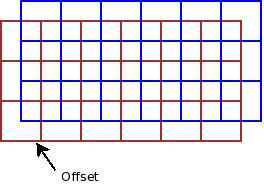
\includegraphics[width=0.3\textwidth]{Domain-mcip-offset.jpg}
	\caption{Example of shifted grids due to one grid being defined by
the grid centre, and the other by the lower left corner.}
	\label{offset}
\end{figure}

Note that \code{.encode('ascii')} on many of the inputs.  This is because by
default ArcGIS returns text in a UTF encoding.  When file names are encoded in
a UTF format, access those files on the file system can then be tricky.

\subsection{Uploading the \ioapi~file}

\singlespace
\begin{minted}[linenos,firstnumber=115]{python}
arcpy.AddMessage("Sending IOAPI file to webservice to repair spatial information")
arcpy.AddMessage("Uploading %s..."%Input_netCDF_File)
params = {'shift_cells':('1' if shift_cells else '0'), \
	'file':open(Input_netCDF_File, 'rb')}

fileName = download(UPLOAD_URL, params, REPAIRED_IOAPI_FILE)
if os.access(fileName, os.R_OK):
	arcpy.AddMessage("Downloaded file: %s"%fileName)
else:
	arcpy.AddMessage("Repaired IOAPI file was not downloaded!")
	raise Exception("Temporary file %s wasn't downloaded!"%fileName)
\end{minted}
\doublespace

This code above calls the custom function \code{download}.  The
function is pass the current \ioapi~file, all required parameters and
downloads a \netcdf~file with the spatial information intact.

\subsection{Generating the Raster File}

\singlespace
\begin{minted}[linenos,firstnumber=146]{python}
arcpy.MakeNetCDFRasterLayer_md(REPAIRED_IOAPI_FILE, Variable, X_Dimension, \
	Y_Dimension, raster_name, "", "", "BY_VALUE")
\end{minted}
\doublespace

Once the \netcdf~file is downloaded from the server, the script calls the \code{MakeNetCDFRasterLayer\_md} tool to generate the raster file.

\subsection{Adding the Raster Layer to the Data Frame}

%\hl{fix error with which data frame this is loaded on to}
\singlespace
\begin{minted}[linenos,firstnumber=157]{python}
arcpy.AddMessage("Loading raster file to data frame")

# get the map document
mxd = arcpy.mapping.MapDocument("CURRENT")

# get the data frame
df = arcpy.mapping.ListDataFrames(mxd,"*")[0]

# create a new layer
newlayer = arcpy.mapping.Layer(raster_name)

# add the layer to the map at the bottom of the TOC in data frame
arcpy.mapping.AddLayer(df, newlayer, "BOTTOM")
\end{minted}
\doublespace

Once the raster file is generated, the code above is used to append it
to the first data frame\footnote{In future versions, this will be
changed to add the layer to the active Data Frame}.

\section{Webservice Code}

The webservice code is written in Python and is run via
\emph{mod\_python} in Apache.  The host server is a Darwin OS X system,
thus all the required software to work with \ioapi~files can be
installed with one command (the same is especially true for Ubuntu
Linux systems.)  This makes it a perfect candidate for a server to
perform these specialized operations compared to running them on the
MS Windows system running ArcGIS.

The server script operates by first parsing the HTTP request made by the client
script, reading the uploaded \ioapi~file, writing spatial information to it,
and returning the new file.  The \ioapi~file is accessed using the open source
\netcdf 4-Python module\footnote{Available at
\url{http://code.google.com/p/netcdf4-python/}}.

The following code sections are shown to illustrate how the information was
written.  The information is written as per the \netcdf~CF Conventions.  Note
that the variable \code{nc} is the original file, while the variable \code{nnc}
is the new file that is being repaired.

\subsection{Writing the Projection Information}

Data in \netcdf~files is not restricted to a single projection, every variable
could have a separate projection.  This is done by declaring a \netcdf~variable
per projection.  In our file, we declare a \ac{lcc} variable. 

Currently this projection is the only projection this script is
capable of authoring projection information for.  However, the script
can be expanded to read the global attribute \code{GRIDTYPE} in
\ioapi~files to determine the projection in use. Because \ac{lcc} is
the most common projection used by \ac{cmaq}, and is used for all the
examples in this tutorial, for now it is hard coded into the script.

\singlespace
\begin{minted}[linenos,firstnumber=134]{python}
try:
	# Lets create the projection variable
	lcc=nnc.createVariable('Lambert_Conformal', 'i4')
	lcc.grid_mapping_name="lambert_conformal_conic"
	lcc.standard_parallel=[nc.P_ALP, nc.P_BET]
	lcc.longitude_of_central_meridian=nc.P_GAM
	lcc.latitude_of_projection_origin=nc.YCENT
	lcc.false_easting = 0.0
	lcc.false_northing = 0.0
except ValueError as (errno, strerror):
	# ...
\end{minted}
\doublespace

In the code above, a dimensionless integer variable is being created with the \netcdf 4-Python module.  The values such as \code{nc.P\_ALP} are \ioapi~attributes on the original \ioapi~file.

\subsection{Adding Spatial Information to Variables}

Now that a projection is defined, each variable to be projected with it must be set as such,

\singlespace
\begin{minted}[linenos,firstnumber=134]{python}
try:
	for var in nc.variables:
		varname = str(var)
		nnc.variables[varname].grid_mapping = 'Lambert_Conformal'
except RuntimeError, err:
	stderr += ('Ack!  RuntimeError: %s\n' % str(err))
\end{minted}
\doublespace

This code loops through all the variables in the file assigning the projection
information that we defined above to the variable attribute
\code{grid\_mapping}.  Note that this is over all the variables, this is
because the script \emph{assumes} that all variables will use the same
projection.  This assumption is justified as \ioapi~files are constrained to
only containing data for one projection.

\subsection{Defining Columns and Rows}

ArcGIS requires $X$ and $Y$ dimensions to generate the raster file, our script
writes that information to the one-dimensional float variables \code{COL} and
\code{ROW} respectively.

\singlespace
\begin{minted}{python}
# Add col/row variables
try:
	col_var=nnc.createVariable('COL', 'f4', ('COL',))
	col_var.units = "km"
	col_var.long_name = "x coordinate of projection"
	col_var.standard_name = "projection_x_coordinate"
	if verbose:
		stdout += "Added COL variable"
except ValueError as (errno, strerror):
	# ...


try:
	row_var=nnc.createVariable('ROW', 'f4', ('ROW',))
	row_var.units = "km"
	row_var.long_name = "y coordinate of projection"
	row_var.standard_name = "projection_y_coordinate"
	if verbose:
		stdout += "Added ROW variable"
except ValueError as (errno, strerror):
	# ...
\end{minted}
\doublespace

These variables define the offset of every cell.  This means that -
with this implementation at least - there is no attribute that defines
the sizes of each cell\footnote{A newer version of this script
experimented with added the \emph{cell\_measures} data defined in the
CF Conventions, however these attempts have to date been unsuccessful}.

The data for these variables is again based on the attributes in the
\ioapi~file.

\singlespace
\begin{minted}{python}
# Populate row/col vars
ncols = len(nc.dimensions['COL'])
nrows = len(nc.dimensions['ROW'])

yorig=nc.YORIG
xorig=nc.XORIG
cellsize=nc.XCELL

cols = numpy.arange(xorig, xorig + (cellsize*ncols), cellsize)
rows = numpy.arange(yorig, yorig + (cellsize*nrows), cellsize)

try:
	col_var[:] = cols;
	row_var[:] = rows;
except IndexError, err:
	# ... 
\end{minted}
\doublespace

\section{Reviewing Spatial Information in ArcGIS}

At this point, the file should include full spatial information.  To confirm
this, once the file is loaded into ArcGIS as a raster layer, on the
layer \textbf{Properties} $\rightarrow$ \textbf{Source} tab, the
\textbf{Spatial Reference} data, as well as all other data (cell size,
extent) should now be filled out.  An example is shown in figure
\ref{confirm_spatial_info_ex}.

\begin{figure}
	\centering
	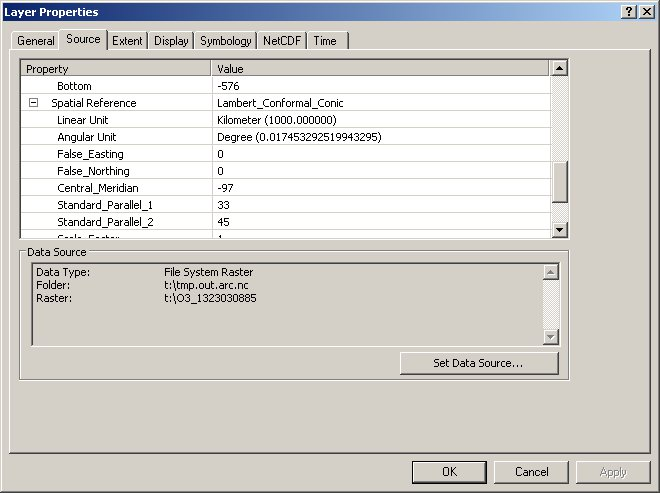
\includegraphics[width=0.60\textwidth]{confirm_spatial_info.jpg}
	\caption{Layer source information dialog}
	\label{confirm_spatial_info_ex}
\end{figure}

\section{Adding Tool Help}

Adding Tool Help is a special challenge in ArcGIS v10.  Tool Help and
other metadata can be added by right clicking on the tool in Arc
Toolbox and selecting \emph{Item Description}.  You will however
notice that there is no place to enter parameter description (help for
each input.)  To do this, you must find the toolbox through Arc
Catalogue through the folder connections tree, not the Toolboxes tree.

Once here, right-click and select \emph{Item Description} again, now
your description editor will have a place to enter parameter help.

Note, if you have already modified the tool description through the
direct way, it will now have been erased.  Also note that now that
this has been done, parameter help can be edited in the \emph{Item
Description} on the tool in the Toolbox.

I suspect the roundabout approach here is due to bugs in ArcGIS v10.
